\glsresetall{} 


\chapter{Software Workflow}\label{chap:workflow}

To demonstrate how \gls{pops} may be used, let us walk through setting up
\gls{pops} for the EG-SAT mission. Suppose the customer defines an Area Target
AOI in the Norwegian Sea where they wish Coarse Imaging and Tip-and-Cue Imaging
to be performed. The \gls{aoi} is defined by the points  in
Table~\ref{tab:norway-aoi}. It is the operator’s responsibility to construct an
operations plan for the next week. To do this, they may use \gls{pops} to aid
them in laying out the deterministic aspects of an operations plan.  That
being, determining remote-sensing opportunities, creating a schedule of
observations, validating that schedule, and creating \glspl{ttc} to be uploaded
to the spacecraft. It should be noted that the real-time ground processing of
the data and the generation of new \glspl{ttc} for the next pass of the
Tip-and-Cue Mode are beyond the capabilities of \gls{pops} and this is handled
by separate, mission-specific automatic ground processing.

\begin{table}[h] 
    \centering
    \caption{Area of Interest Definition}
    \begin{tabular}{cccc}
	Point                  & Latitude [$^\circ$] & Longitude [$^\circ$] & Altitude [m] \\ \hline
	\multicolumn{1}{l|}{0} & 73       & -20      & 0        \\
	\multicolumn{1}{l|}{1} & 66       & 19       & 0        \\
	\multicolumn{1}{l|}{2} & 78       & 41       & 0        \\
	\multicolumn{1}{l|}{3} & 82       & 9        & 0        \\
	\multicolumn{1}{l|}{4} & 79       & -17      & 0       
    \end{tabular}
    \label{tab:norway-aoi}
\end{table}

Each step in this process makes use of menus and forms in \gls{pops} that a
user can fill out. To avoid having an excessive number of screenshots for each
step, the input data itself will mostly be shown in tables or figures rather than
through screenshots of the menus.

\subsection{Plan Configuration}

First, \gls{pops} must be configured for a particular mission. The operator
must specify the mission, its satellites, satellite sensor parameters, and its
available ground stations. This will only need to be set once per mission. For
our example scenario, the mission is EG-SAT, the satellites are Sat-A and
Sat-B, and the ground station is the \gls{sfl} in Toronto. The relevant payload
sensors must be specified for each satellite. These are the sensors that affect
payload observations and are referenced by the Opportunity Filter. Currently,
the sensor information is very simple but in the future, this system will be
more developed as \gls{pops}'s modeling capabilities are improved. The sensor
information for Sat-A and Sat-B can be seen in Table~\ref{tab:sensors}. 

\begin{table}[h] 
    \centering
    \caption{Sensor Definitions}
    \begin{tabular}{ccc}
	Satellite                  & Sensor Name & Parameters    \\ \hline
	\multicolumn{1}{l|}{Sat-A} & Coarse      & \{"FOV": 60.0\} \\
	\multicolumn{1}{l|}{Sat-B} & Fine        & \{"FOR": 20.0\}
    \end{tabular}
    \label{tab:sensors}
\end{table}

Relevant ground stations should also be added into \gls{pops}. For each
station the name, location, and elevation mask should be specified. The
location is just in Latitude-Longitude-Altitude. The elevation mask specifies
at what angle, from the horizon, does an object in space become visible; This
is approximated as a single angle. The minimum value for the mask is $0^\circ$,
which is when there are no obstructions at all. For larger mask values, the
less a ground station is able to observe. For EG-SAT, only \gls{sfl} will be
added. Its parameters can be seen in Table~\ref{tab:ground-stations}. It should
be noted that the elevation mask is just an example value.

\begin{table}[h] 
    \centering
    \caption{SFL Ground Station}
    \begin{tabular}{ccccc}
	Station                  & Latitude [$^\circ$] & Longitude [$^\circ$] & Altitude [m] & Elev. Mask [$^\circ$] \\ \hline
	\multicolumn{1}{l|}{SFL} & 43.78   & -79.47   & 193.0  & 10      \\
    \end{tabular}
    \label{tab:ground-stations}
\end{table}

After this is done, the operator will then start creating a plan. Plans lay out
the scenario from which an operator can search for observations and add
them to the schedule. Plan creation begins by specifying the
\glspl{tle} for each satellite.  These can be previous \glspl{tle} stored in
the \gls{pops} database, new \glspl{tle} taken from CelesTrak or Spacer-Track,
or custom-made \glspl{tle} that may be used for simulation or may be more
accurate \glspl{tle} derived from a spacecraft’s onboard \gls{gps} ephemeris.
Once the \glspl{tle} are selected, Ephemerides are generated for each satellite and
stored in the database. For the EG-SAT scenario, \glspl{tle} were generated
with the \gls{stk}. A current limitation of \gls{pops} is that once \glspl{tle}
are selected for a plan, they cannot be changed. Allowing \glspl{tle} to be
changeable would make far too complicated at this stage of development so this
will be addressed in future revisions. For EG-SAT, we will use the \glspl{tle}
in Figure~\ref{fig:tles}.

\begin{figure}[h]
    \begin{verbatim}
    SAT-A
    1 99999U 18099H   24015.66666667  .00000264  00000-0  11261-4 0  0003
    2 99999  96.4575 096.8235 0010629 287.9022 255.6332 15.22959214000011

    SAT-B
    1 99999U 18099H   24015.66666667  .00000265  00000-0  11291-4 0  0007
    2 99999  96.4569 096.8239 0010629 287.8995 250.4360 15.22958218000013
    \end{verbatim}
    \caption{\glspl{tle} For Sat-A and Sat-B}
    \label{fig:tles}
\end{figure}

These \glspl{tle} are artificial and have been created for this scenario. As
such, their NORAD-ID is 9999. Their specifics are not important but, of note,
is that both of their orbits are nearly identical. The only difference being
that the Mean Anomaly of Sat-B is $5^\circ$ less than Sat-A. This means Sat-B
follows the same approximate orbit of Sat-B but it lags behind by some period
of time. Also of note is the reference epoch of both \glspl{tle}, ``2024-01-15
16:00:00.000''.

Once the \glspl{tle} have been selected and confirmed. Ephemerides must be
generated for each satellite in the plan. To do this, the start and end epochs
must be specified, as well as the step size of the propagation. Propagating
\glspl{tle} is generally only accurate $\pm 2$ weeks from the reference epoch
of the \gls{tle}. They may be accurate for more or less time on a case-by-case
basis but, for now, \gls{pops} sets a limit of 2 weeks from the reference epoch
for ephemerides. Any time later or earlier is likely to be inaccurate.
Currently, the step size must be set for the entire scenario. This has become
an issue and will need to be addressed in the future. For long scenarios, such
as 1-2 weeks, having a small step size will yield a large amount of data that
needs to be stored. For a 2 week scenario, at a 10s timestep, one satellite
ephemeris has 120,960 points.  Where each point contains 3 floats for position,
3 floats for velocity, and an epoch string. Some scenarios may have multiple
satellites and this increases the amount of data exponentially. So, for long
scenarios, having a small timestep is not ideal. If a larger timestep is used,
then the opportunity filtering may become less accurate because there is less
information. In the future, more sophisticated methods of ephemeris generation
that better handle data usage will be developed but for now, the step size is
constant for a whole scenario. For EG-SAT, we will create a 3 day scenario
starting at the reference epoch with a 10 second timestep. 

Before continuing, we must also specify what ground stations are relevant to a
plan. Earlier, a ground station was added to \gls{pops} but here we must
associate it with the plan. The reason for doing it in this way is that there
may be scenarios where a mission has a constrained set of potential ground
stations, or other ground stations may become available. Associating ground
stations with a plan allow for them to be configurable. 

Once these settings are confirmed, ephemeris data is generated for each
satellite in the mission and this data is stored in the database. The access
times for each ground station are also calculated for each satellite and that
data is stored as well.


\subsection{Observation Configuration Webpage}

\begin{figure}[h]
    \centering
    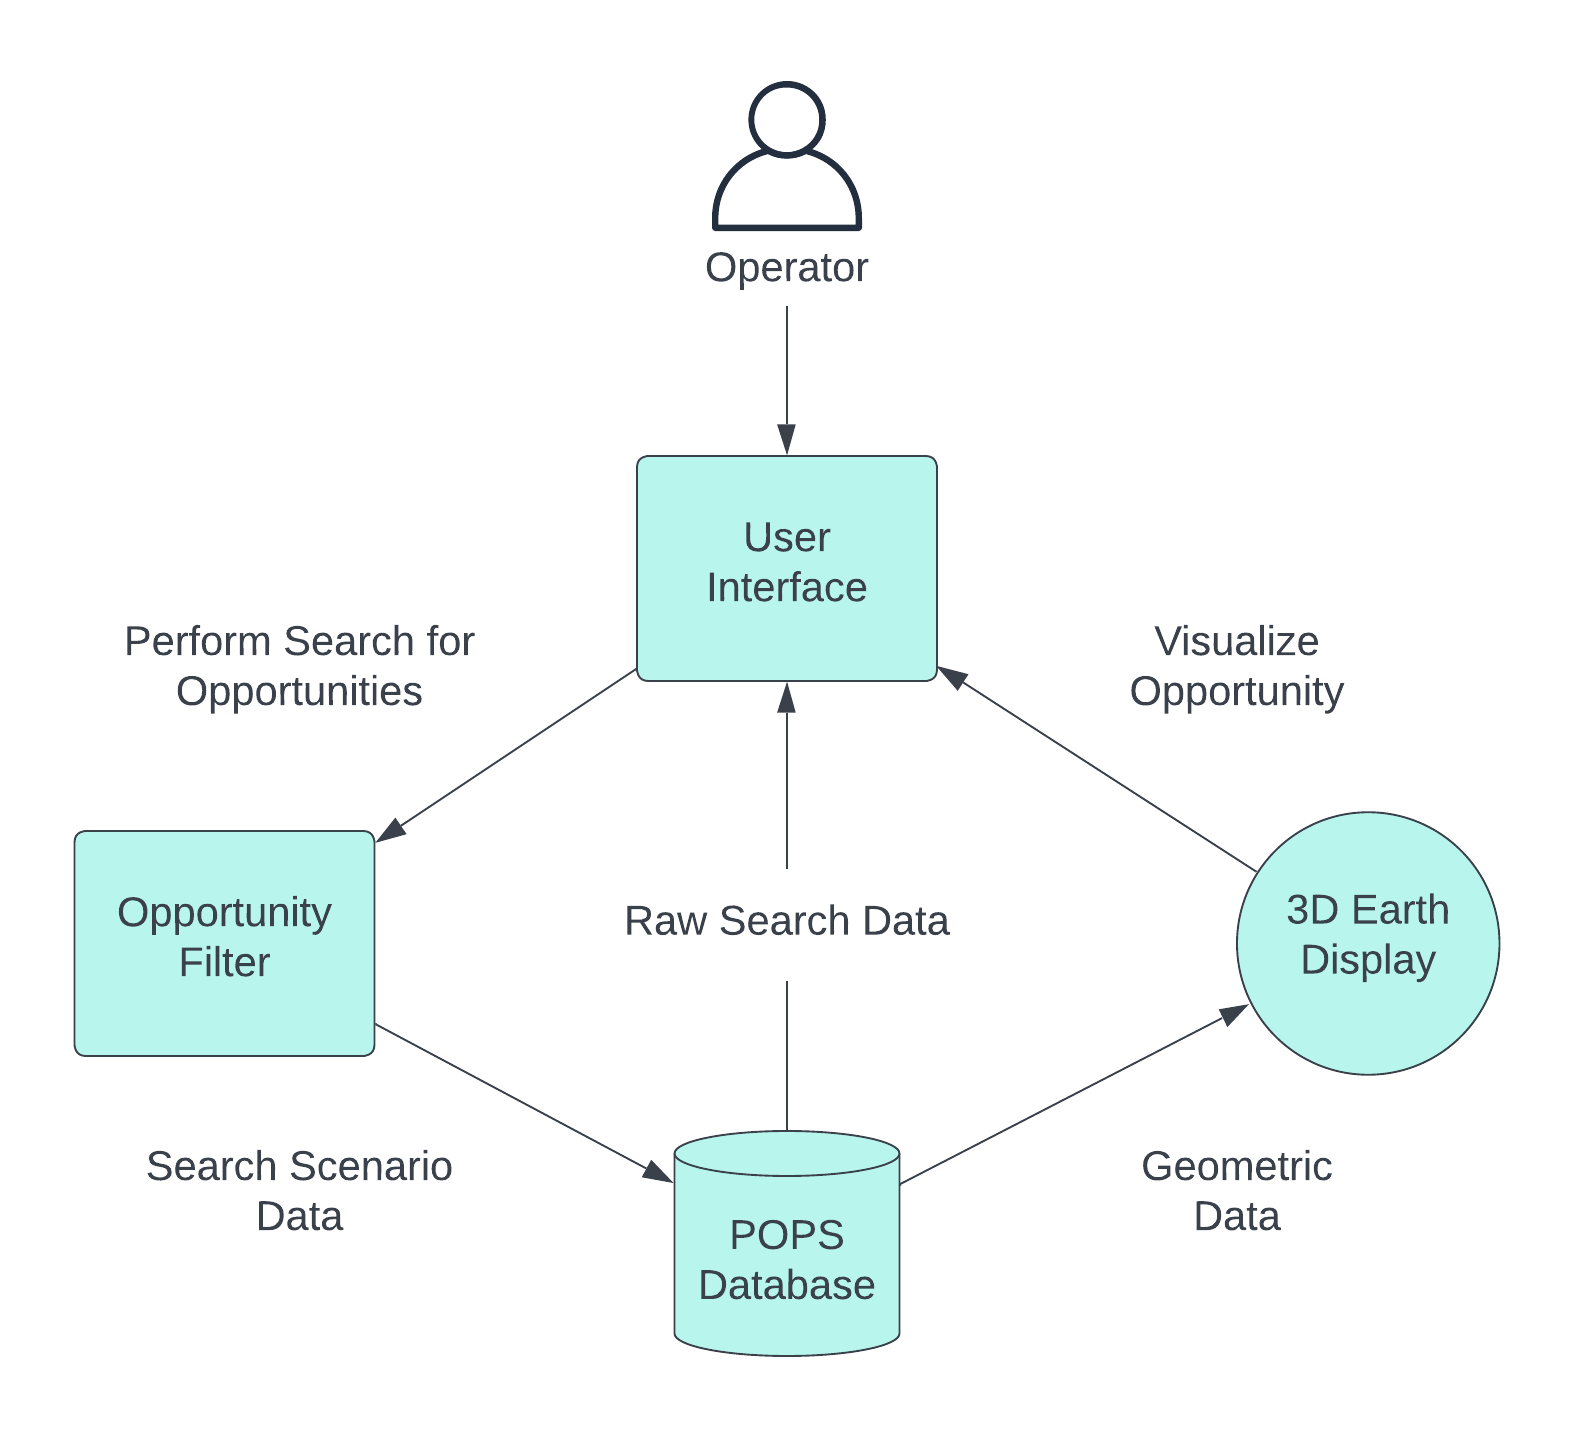
\includegraphics[width=0.5\textwidth]{opp_search_flow.png} 
    \caption{Observation Filtering Summary}
    \label{fig:obs_fil} 
\end{figure}

Once our scenario is set up, we begin Observation Configuration. \gls{pops}
must display potential observation opportunities to the user and must enable
the user to create observations based on these potential opportunities.
Opportunity filtering is the process of taking a large set of potential
observations and constraining them to an \gls{aoi}. Observations can be
performed anywhere on Earth, but we only care about those that provide useful
data for our operations strategy.  The basic process for displaying
opportunities to the user can be seen in Figure~\ref{fig:obs_fil}. An operator
first creates a search scenario through the \gls{gui}.  For a given mission,
there may be multiple observation types, multiple possible \glspl{aoi}, and a
combination of one or more satellites that are part of the observation. All of
this is specified by the user in the form of a search scenario. These
parameters are fed to the Opportunity Filter which generates search data.
Rather than having the search data displayed immediately, all of the generated
search data is stored in the database. From here, it can be retrieved at any
time, without needing to re-compute a search scenario. Some raw search data may
be retrieved and displayed directly to the \gls{gui}. Mostly, these are just
access times.  Alternatively, the raw data may undergo further processing to be
displayed in the 3D Earth visualization. Currently, satellites, satellite
trajectories, ground stations, ground access times, \glspl{aoi}, and swaths can
be displayed.


Since an operator will spend most of their time on the Observation
Configuration page, we shall spend some time discussing it and the utilities
provided with the page. It should be emphasized that \gls{gui}  development is
difficult. A good \gls{gui} and a bad \gls{gui} can functionally do the same
thing but the good \gls{gui} will be easier to use, robust, and visually
pleasing. What's more is that they are extremely time-consuming; hours can be
spent on just a single button, for example. The goal for \gls{pops} is not to
create the perfect user interface but rather the actual functionality itself,
time spent on the webpages themselves is minimized in favor of creating a
functional product. 

\begin{figure}
    \centering
    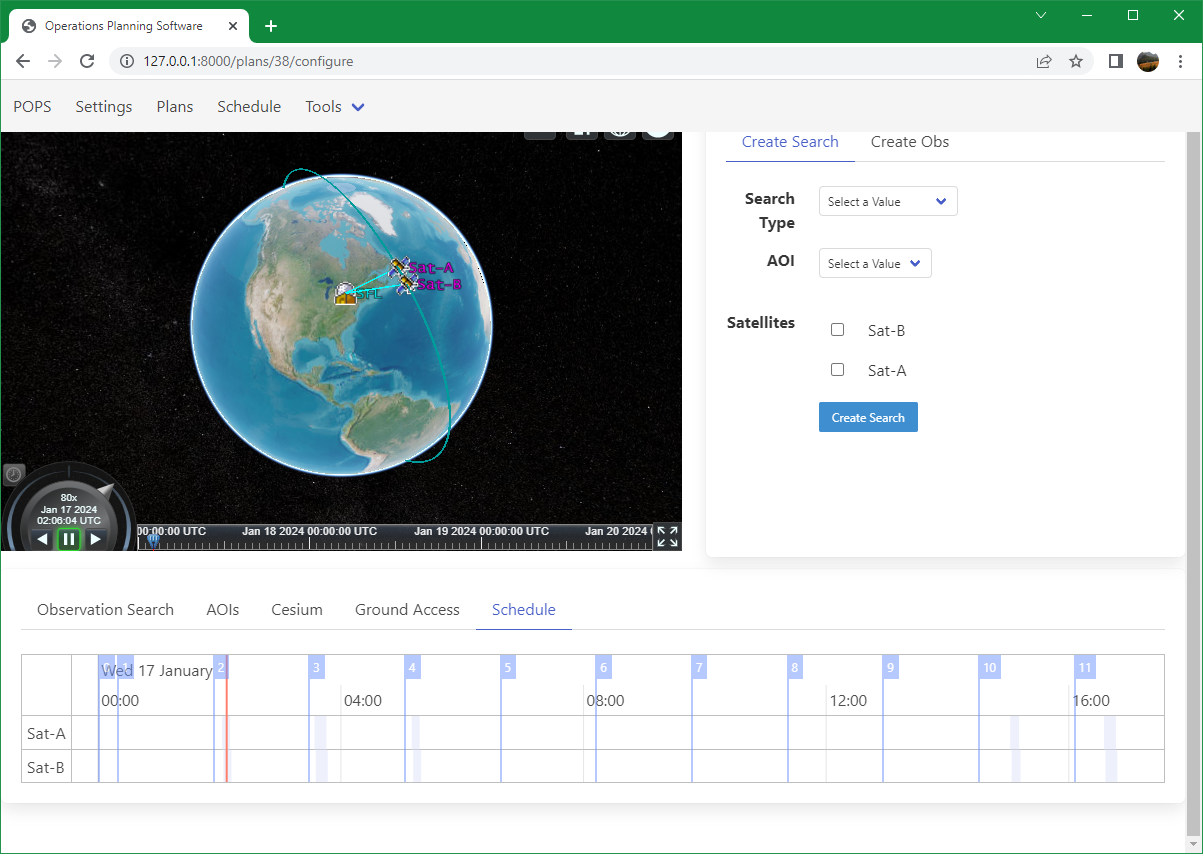
\includegraphics[width=0.8\textwidth]{obs-conf-base.png} 
    \caption{Observation Configuration Webpage}
    \label{fig:obs-conf-base} 
\end{figure}


With that in mind, the Observation Configuration page can be seen in
Figure~\ref{fig:obs-conf-base}. The Cesium viewer is located on the top left of
the page.  There, an operator can see: the Earth, the satellites, their
trajectories, possible ground access times, an Area of Interest, and potential
observation opportunities. In the top right are forms that the user can fill
out to add or make changes to the plan. Currently, that consists of forms to
create search scenarios or to add observations to the plan. The bottom tabs are
meant to display information to the user or allow them to interact with the
Cesium viewer. Currently visible, in the bottom is the schedule timeline.
Here, events are displayed to the user in an intractable viewer. Before going
through how the page is used, the different aspects of the page will be touched
on briefly. 


\begin{figure}[h]
    \centering
    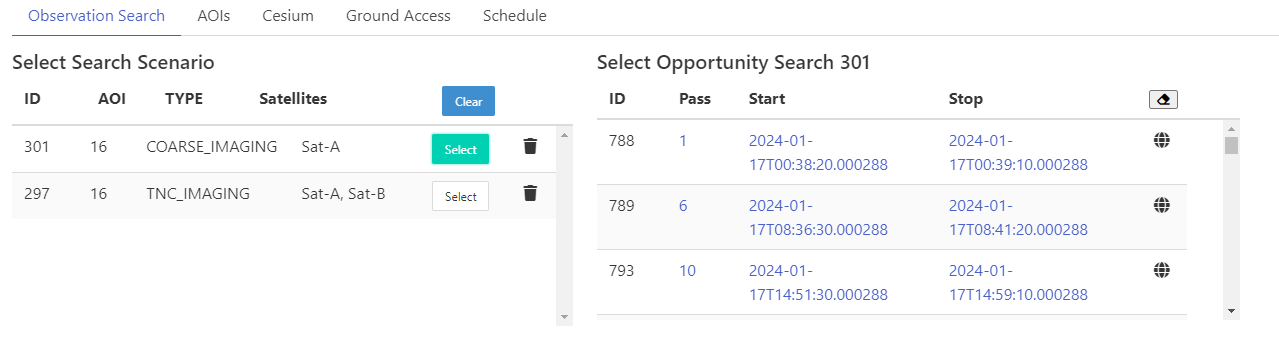
\includegraphics[width=0.8\textwidth]{obs-conf-search.png} 
    \caption{Observation Search Tab}
    \label{fig:obs-conf-search} 
\end{figure}

The results of a search can be seen in the observation search tab in
Figure~\ref{fig:obs-conf-search}. This tab is split into two lists. The left
list displays a list of the search scenarios that are associated with the plan.
When a new search scenario is added, it is added to this list. Here, search
scenarios can be deleted with the trash icon or they may be displayed in the
viewer. For a selected search scenario, the right list displays all of the
opportunities associated with it. Information such as the pass index of the
opportunity, start epoch, and end epochs are displayed to the user. The blue
text entries are hyperlinks. When clicked, they update the current time of the
Cesium viewer. For example, for opportunity \texttt{788} (these are global IDs
not search scenario IDs) if the user clicks on the start epoch, the viewer will
change time to 12:38 AM Jan 17, 2024. The globe icon on the right allows a user
to display or hide an opportunity. Similarly, the eraser icon in the header
toggles the visibility of all opportunities.  The usefulness of these can be
seen in Figure~\ref{fig:obs-conf-ci}.  In Figure~\ref{fig:obs-conf-ci-1},
all of the opportunities in the scenario are displayed. This is of course quite
messy and difficult to understand. In Figure~\ref{fig:obs-conf-ci-2} all of
the opportunities in the scenario have been hidden except for two
opportunities. This makes it far easier to select only the opportunities that
are of interest to an operator.


\begin{figure}[h]
    \centering
    \begin{subfigure}[b]{0.49\textwidth}
	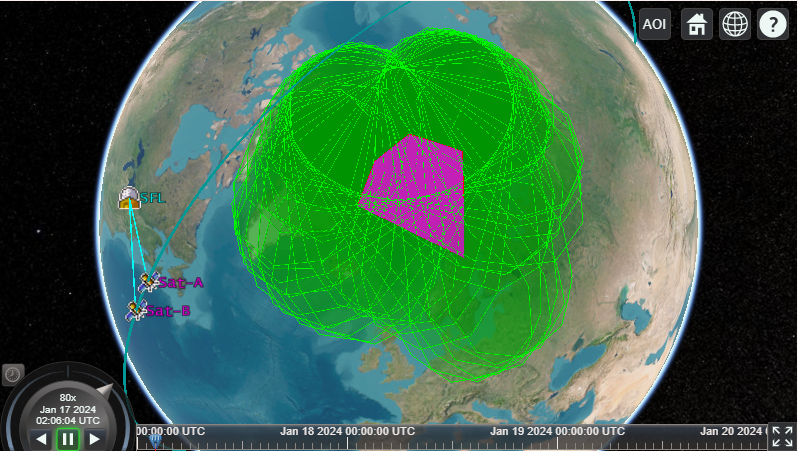
\includegraphics[width=\textwidth]{obs-conf-ces-coarse-1.PNG} 
	\caption{All Opportunities}
	\label{fig:obs-conf-ci-1} 
    \end{subfigure}
    \hfill
    \begin{subfigure}[b]{0.49\textwidth}
	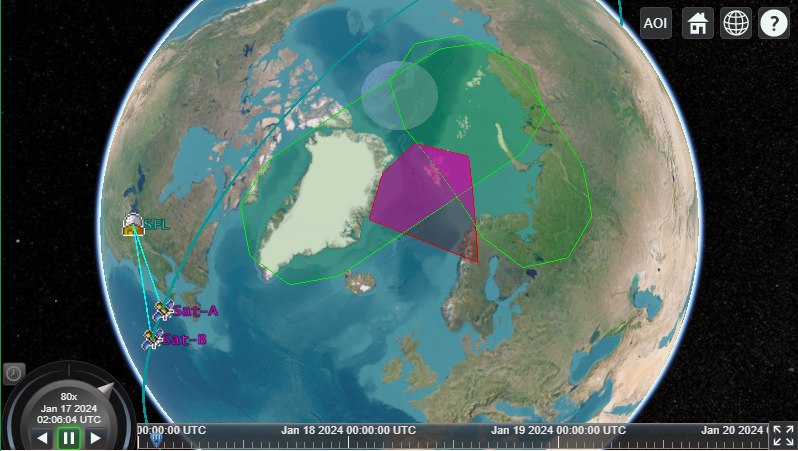
\includegraphics[width=\textwidth]{obs-conf-ces-coarse-2.PNG} 
	\caption{Two Opportunities}
	\label{fig:obs-conf-ci-2} 
    \end{subfigure}
    \caption{Opportunities Displayed in Cesium}
    \label{fig:obs-conf-ci} 
\end{figure}

Every \gls{aoi} that is stored in \gls{pops} can be seen in the \texttt{AOI}
tab. \glspl{aoi} May be added either through a text file that is read and
loaded into \gls{pops}. Alternatively, \glspl{aoi} can be drawn directly in the
Cesium viewer with the \texttt{AOI} button in the Cesium viewer. When it is
clicked, the controls for the viewer change. Every time a user clicks on the
Earth, a polygon vertex is placed at that location. As vertices are added a
white polygon becomes visible. If a mistake is made, the user can undo vertices
by pressing \texttt{CTRL-Z}. To give the user more information, some
instructions are included in a text box as well as the Latitude and Longitude
of the cursor.  Once the user is satisfied, they can right click and the
area-target \gls{aoi} is saved to the database and can be referenced by search
scenarios. A Partially completed \gls{aoi} can be seen in
Figure~\ref{fig:obs-conf-draw}. 

\begin{figure}
    \centering
    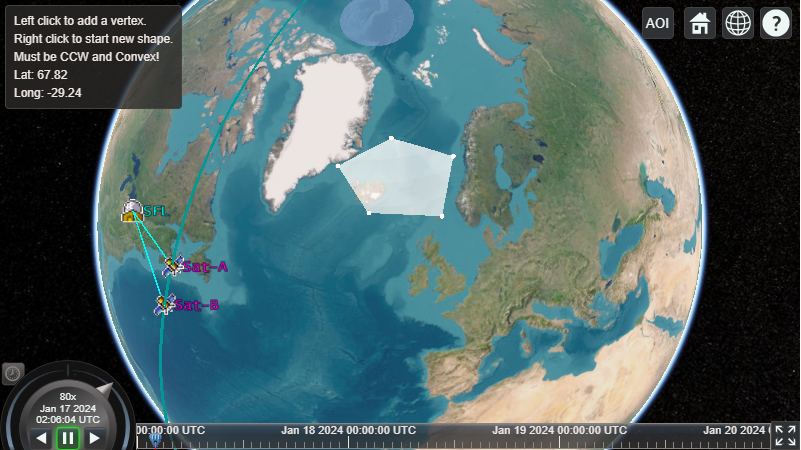
\includegraphics[width=0.8\textwidth]{obs-conf-draw.png} 
    \caption{Drawing an AOI}
    \label{fig:obs-conf-draw} 
\end{figure}

Since there may be many \glspl{aoi} stored in \gls{pops}, a user can display
\glspl{aoi} in the Cesium viewer from the \texttt{AOI} tab. This can be seen in
Figure~\ref{fig:obs-conf-aoi-display}. These `displayed' \glspl{aoi} have red
outlines and purple areas. This is to distinguish them from \glspl{aoi} that
are displayed as part of a search scenario. A useful feature of Cesium is also
viewable in the Figure. When an entity in Cesium is selected, an information
box appears giving the name of the entity as well as its description. Here, the
\gls{aoi} has no description, but from the name, we can tell its: an \gls{aoi},
its ID is \texttt{16}, and it is a display \gls{aoi}.

\begin{figure}[h]
    \centering
    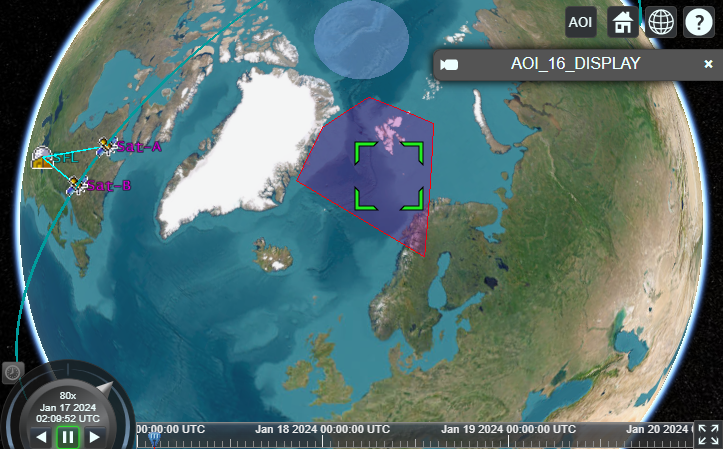
\includegraphics[width=0.8\textwidth]{obs-conf-aoi-disp.png} 
    \caption{Displaying an AOI}
    \label{fig:obs-conf-aoi-display} 
\end{figure}

The last two tabs serve minor purposes. The \texttt{Cesium} tab lists all of
the currently loaded objects in the Cesium Viewer. It allows a user to display
or hide any object. This is mostly useful for debugging, or if a user wants a
specialized view. For example, they may wish to show the intersection polygons
from a number of opportunities. Alternatively, they may wish to compare swaths
from different passes. This tab gives the user the granular ability to make
those changes. The \texttt{Ground Access} tab shows a filter-able list of
ground station accesses, with time links that change Cesium's current time.


\subsection{Searching For Opportunities}

Let us now create two search scenarios, one for the Coarse Imaging Operations
mode and one for the Tip-and-Cue Imaging Mode. To do this we will use the
\texttt{Create Search} tab. In this form, we must specify the search type, the
\gls{aoi} the search should be conducted on, and the  satellites that should be
considered. The search type may be selected from the dropdown. If a user
is unsure about what ID their desired \gls{aoi} is given, they can go to the
\texttt{AOI} tab. There, they may look at the list of \glspl{aoi} and display
them on Cesium for their reference. Earlier in the chapter, an \gls{aoi} was
specified by the imaginary customer in Table~\ref{tab:norway-aoi}. A text file
for this \gls{aoi} definition was written and then uploaded to \gls{pops}. The
ID that was generated was \texttt{16}. This \gls{aoi} can actually be seen
displayed earlier in Figure~\ref{fig:obs-conf-aoi-display}.

\begin{figure}[h]
    \centering
    \begin{subfigure}[b]{0.49\textwidth}
	\centering
	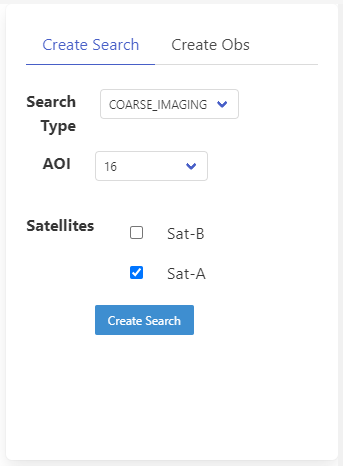
\includegraphics[width=0.60\textwidth]{obs-conf-search-1.PNG} 
	\caption{Coarse Imaging Settings}
	\label{fig:obs-conf-search-1} 
    \end{subfigure}
    \hfill
    \begin{subfigure}[b]{0.49\textwidth}
	\centering
	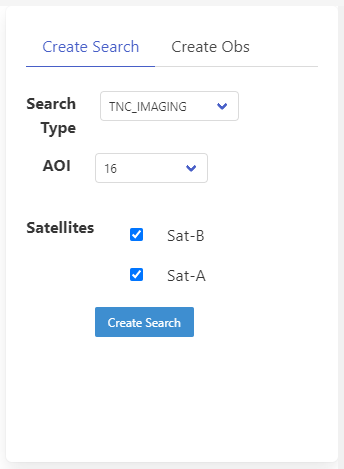
\includegraphics[width=0.60\textwidth]{obs-conf-search-2.PNG} 
	\caption{Tip-and-Cue Imaging Settings}
	\label{fig:obs-conf-search-2} 
    \end{subfigure}
    \caption{Search Scenario Form Parameters}
    \label{fig:obs-conf-searches} 
\end{figure}


For Coarse Imagine the search mode is, of course, \texttt{COARSE\_IMAGING}.
The satellites of relevance for this mode is just Sat-A, because Sat-B is not
equipped with a Coarse Imager. In the future, only relevant satellites will be
selectable but, for now, it is left configurable.  The search form for this
mode can be seen in Figure~\ref{fig:obs-conf-search-1}. Similarly, for
Tip-and-Cue imaging, the mode is \texttt{TNC\_IMAGING} the relevant satellites
are Sat-A and Sat-B.  The mode's settings can be seen in
Figure~\ref{fig:obs-conf-search-2}. Once the \texttt{Create Search} button is
clicked, \gls{pops} will send the data to the Opportunity Filter and a search
will be performed. The two searches can be seen in the \texttt{Observation
Search} tab in Figure~\ref{fig:obs-conf-search}. In the Figure, note that: the
swaths are displayed with green outlines and faint green areas. The \gls{aoi}
has a red outline and a black area, and the intersection polygons have magenta
areas. The Coarse Imaging search mode can be seen in
Figure~\ref{fig:obs-conf-ci}. In total,
there are 43 opportunities for this mode in a 72 hour period. The reason there
are so many is that there are not many constraints for this kind of
observation. All the mode is is a single access time to an area target. 

\begin{figure}[h]
    \centering
    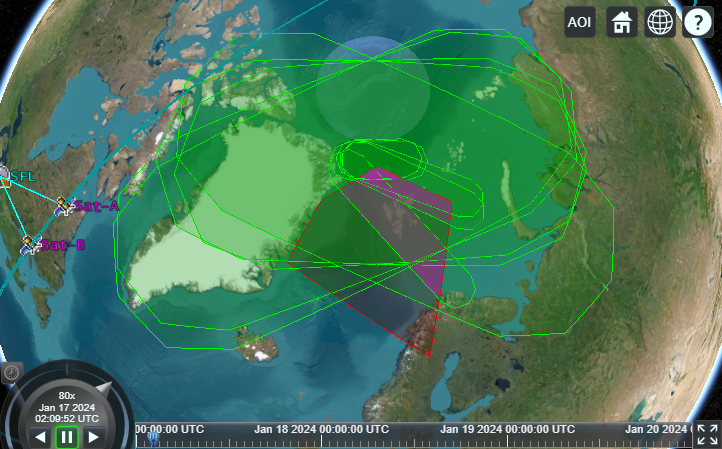
\includegraphics[width=0.7\textwidth]{obs-conf-tnc-all.png} 
    \caption{Tip-and-Cue Imaging All opportunities}
    \label{fig:obs-conf-tnc-all} 
\end{figure}

In contrast, all the opportunities for Tip-and-Cue Imaging mode can be seen in
Figure~\ref{fig:obs-conf-tnc-all}. This view is a bit cluttered but there are
not many opportunities, so individual screenshots have been taken for each
opportunity in Figure~\ref{fig:obs-conf-tnc-opps}. The way each opportunity is
displayed is with two swaths.  The tip swath is the larger one and comes from
Sat-A during the first pass. The cue swath is the thinner swath within the
tip-swath. This comes from Sat-B during the next pass. Note, here the
intersection polygon is the intersection between the tip swath, cue swath, and
\gls{aoi}. For all these opportunities, the tip swath totally encompasses the
cue swath but this is not always the case. In total, there are 5 opportunities
in a 72 hour period. This is far less than there are Course Imaging
opportunities. This is even less than there are general Tip-and-Cue
opportunities. That is, where the cue swath intersects the tip swath and
\gls{aoi}. The reason there are so few opportunities, is because of the ground
station constraint. There must be a ground station contact between the first
pass and next pass. If the satellites are moving from right to left in all of
the views, notice that the tip swaths are all `pointed' at the \gls{sfl} which
is the only ground station. Furthermore, \gls{sfl} is far away from the
\gls{aoi} so opportunities are limited.


\begin{figure}[h]
    \centering
    \begin{subfigure}[b]{0.32\textwidth}
	\centering
	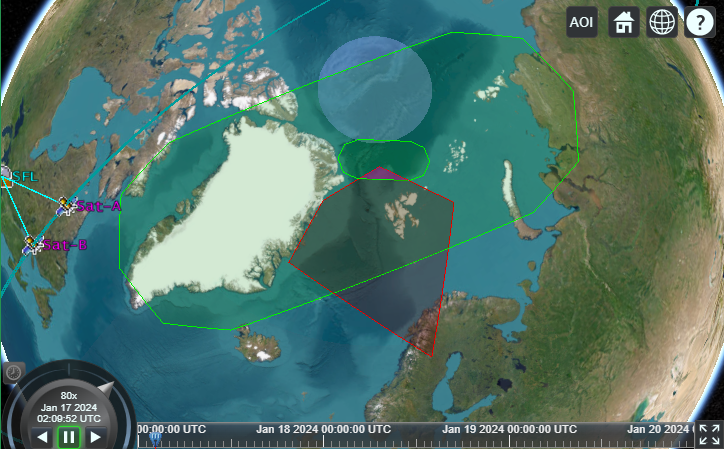
\includegraphics[width=\textwidth]{obs-conf-tnc-1.PNG} 
	\caption{Opportunity 1}
	\label{fig:obs-conf-tnc-1} 
    \end{subfigure}
    \hfill
    \begin{subfigure}[b]{0.32\textwidth}
	\centering
	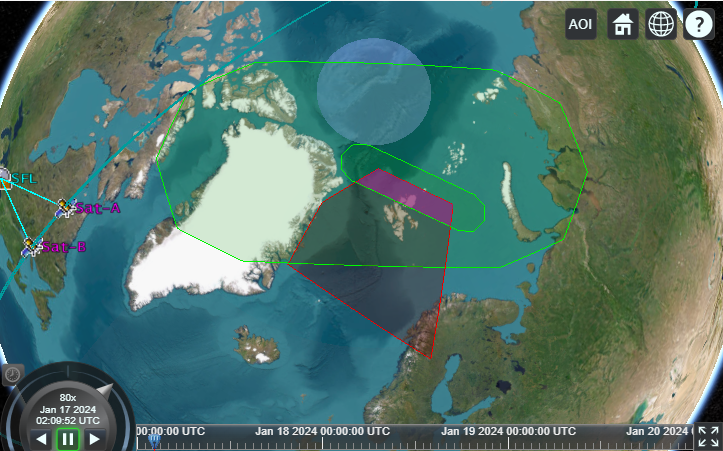
\includegraphics[width=\textwidth]{obs-conf-tnc-2.PNG} 
	\caption{Opportunity 2}
	\label{fig:obs-conf-tnc-2} 
    \end{subfigure}
    \hfill
    \begin{subfigure}[b]{0.32\textwidth}
	\centering
	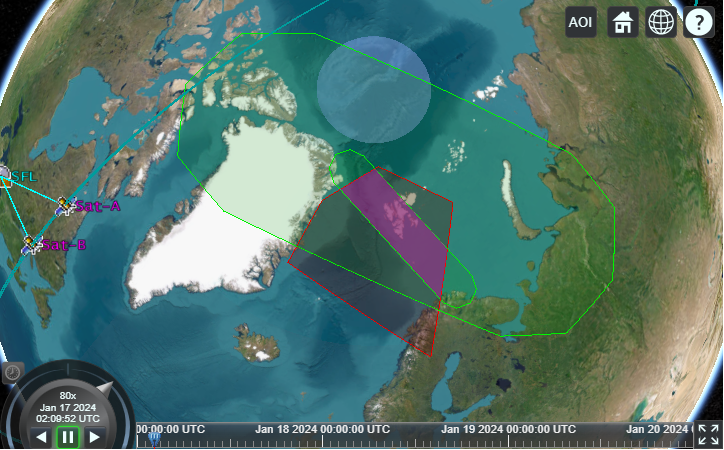
\includegraphics[width=\textwidth]{obs-conf-tnc-3.PNG} 
	\caption{Opportunity 3}
	\label{fig:obs-conf-tnc-3} 
    \end{subfigure}
    
    \begin{subfigure}[b]{0.32\textwidth}
	\centering
	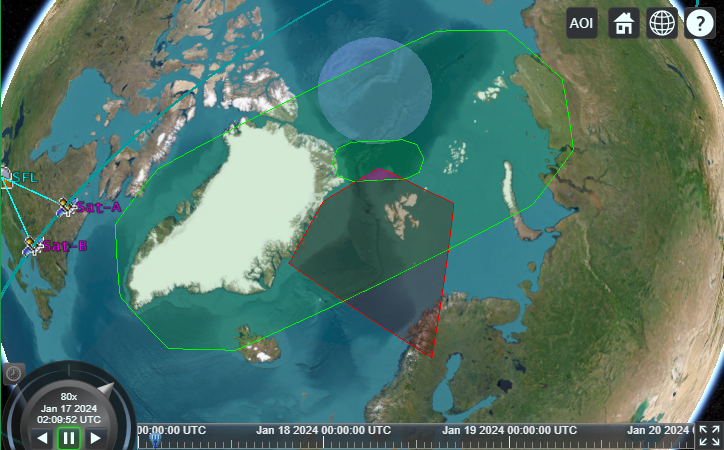
\includegraphics[width=\textwidth]{obs-conf-tnc-4.PNG} 
	\caption{Opportunity 4}
	\label{fig:obs-conf-tnc-4} 
    \end{subfigure}
    \quad \quad
    \begin{subfigure}[b]{0.32\textwidth}
	\centering
	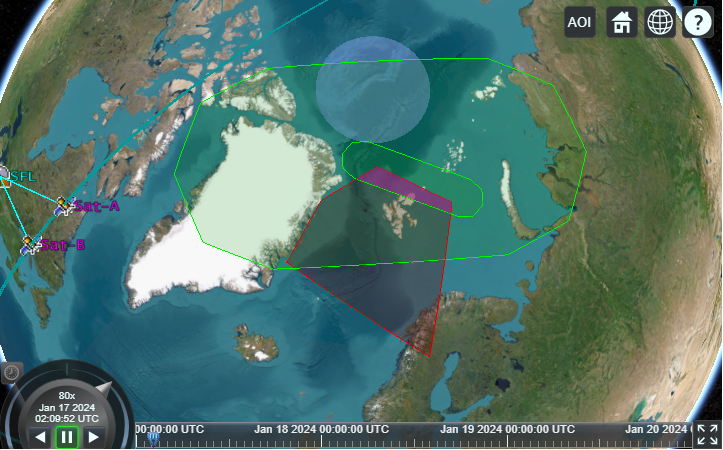
\includegraphics[width=\textwidth]{obs-conf-tnc-5.PNG} 
	\caption{Opportunity 5}
	\label{fig:obs-conf-tnc-5} 
    \end{subfigure}

    \caption{Individual Tip-and-Cue Opportunities}
\label{fig:obs-conf-tnc-opps}
\end{figure}

\begin{table}[h] 
    \centering
    \caption{Plan Summary}
    \begin{tabular}{cc}
	Plan & Stations \\ \hline
	1   &	SFL \\
	2   &	SFL, GSW \\
	3   &	SFL, ESCS 
    \end{tabular}
    \label{tab:additional-plans}
\end{table}

As an example, let us create two more plans with different additional ground
stations, to compare the number of opportunities we can observe. Each plan is
set up identically; the only difference being the ground stations added. If the
plan we have been working with so far is Plan 1, let us create two more plans,
Plan 2 and Plan 3, which have additional ground stations added.  Plan 2 has the
\gls{sfl} and the Weilheim ground station (GSW), near Munich, in Germany. Plan
3 has the \gls{sfl} and the Esrange Space Center Station (ESCS) in Sweden. This
is summarized in Table~\ref{tab:additional-plans}. The parameters for both
these ground stations can be seen in Table~\ref{tab:additional-gs}. The
placements of each ground station with respect to \gls{sfl} and the \gls{aoi}
can be seen in Figure~\ref{fig:obs-conf-gs-placements}. Of course, these are
just example ground stations that have been picked just for this scenario.
Whether they support commercial missions or if they are equipped to support
EG-SAT is not irrelevant. It should be assumed that they can. 

\begin{table}[h] 
    \centering
    \caption{Additional Ground Stations}
    \begin{tabular}{ccccc}
	Station & Latitude [$^\circ$] & Longitude [$^\circ$] & Altitude [m] & Elev. Mask [$^\circ$] \\ \hline
	\multicolumn{1}{l|}{GSW}  & 47.88   & 11.08   & 610.0  & 6      \\
	\multicolumn{1}{l|}{ESCS} & 67.88   & 21.05   & 440.6  & 10      \\
    \end{tabular}
    \label{tab:additional-gs}
\end{table}

\begin{figure}[h]
    \centering
    \begin{subfigure}[b]{0.49\textwidth}
	\centering
	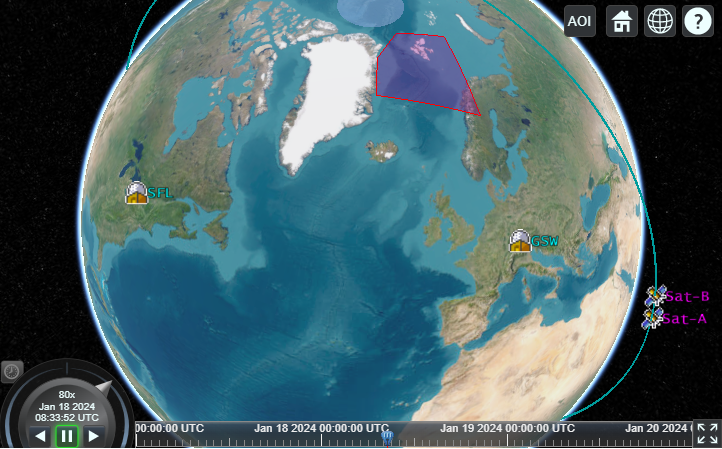
\includegraphics[width=\textwidth]{obs-conf-plan-2.PNG} 
	\caption{Weilheim Station and SFL}
	\label{fig:obs-conf-gs-placements-1} 
    \end{subfigure}
    \hfill
    \begin{subfigure}[b]{0.49\textwidth}
	\centering
	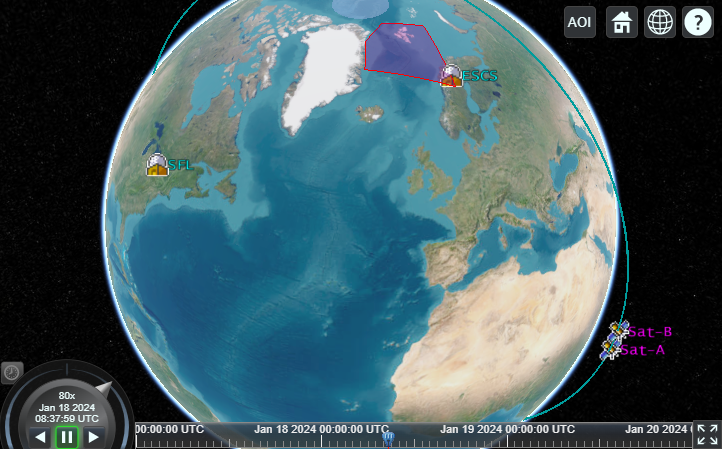
\includegraphics[width=\textwidth]{obs-conf-plan-3.PNG} 
	\caption{Esrange Station and SFL}
	\label{fig:obs-conf-gs-placements-2}
    \end{subfigure}
    \caption{Additional Ground Stations}
    \label{fig:obs-conf-gs-placements} 
\end{figure}

The resulting opportunities can be seen in Figure~\ref{fig:obs-conf-opps}.  For
clarity, the tip swaths have been omitted. As mentioned earlier, Plan-1 only
has 5 opportunities; Plan-2 has 11 opportunities; and Plan-3 has 13
opportunities. It makes sense that with the Weilheim station, more
opportunities will be available since it is located in a different direction
with respect to the \gls{aoi}. Therefore there are accesses for this station
that are not available to \gls{sfl}. The Esrange station happens to be located
very close the \gls{aoi} in this scenario. Therefore, every time the satellites
have access to the \gls{aoi}, it is likely they will also have a ground access
available. 

\begin{figure}[h]
    \centering
    \begin{subfigure}[b]{0.32\textwidth}
	\centering
	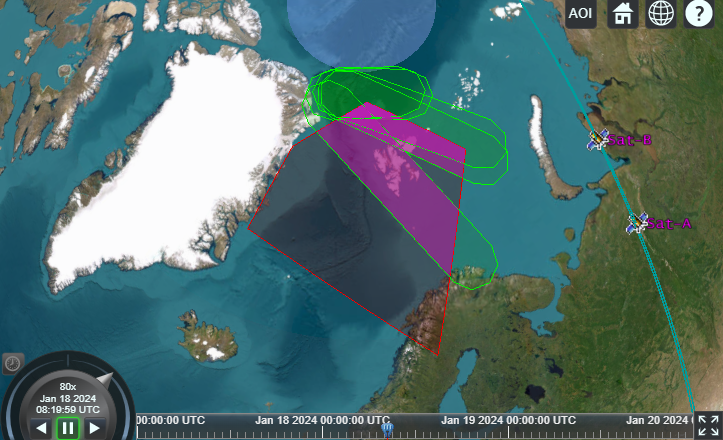
\includegraphics[width=\textwidth]{obs-conf-opps-2.PNG} 
	\caption{Plan 1, 5 Opportunities}
	\label{fig:obs-conf-opps-1}
    \end{subfigure}
    \hfill
    \begin{subfigure}[b]{0.32\textwidth}
	\centering
	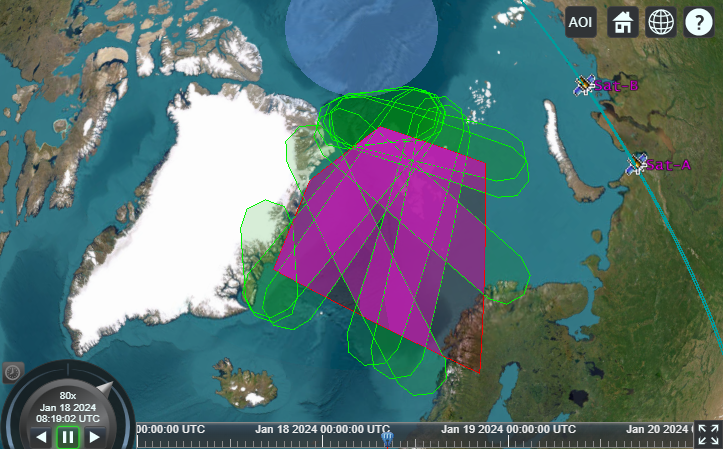
\includegraphics[width=\textwidth]{obs-conf-opps-1.PNG} 
	\caption{Plan 2, 11 Opportunities}
	\label{fig:obs-conf-opps-2} 
    \end{subfigure}
    \hfill
    \begin{subfigure}[b]{0.32\textwidth}
	\centering
	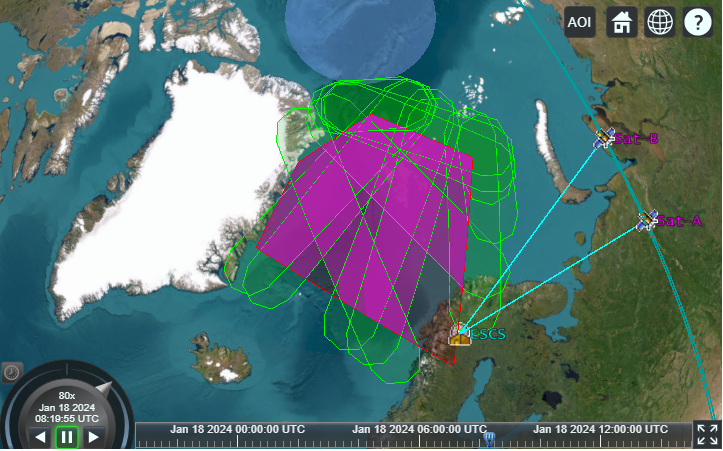
\includegraphics[width=\textwidth]{obs-conf-opps-3.PNG} 
	\caption{Plan 3, 13 Opportunities}
	\label{fig:obs-conf-opps-3} 
    \end{subfigure}

    \caption{Different Plan Opportunities}
    \label{fig:obs-conf-opps}
\end{figure}

For the opportunity filters, there will need to be some fine-tuning going
forward. Edge cases, that were not immediately addressed in their high-level
descriptions or in the actual implementation may have been missed. Questions
like, can one satellite communicate with a ground station while the other is
taking sensor measurements? Are there limitations on ground contacts beyond
just the spacecraft having access? These will be addressed iteratively and the
opportunity filters will be refined through testing and through operations
trials.

\subsection{Creating Observations}

With these opportunities, operators can then create observations. Currently,
this is a manual entry process. An operator must specify both the epoch of an
observation as well as the duration. For the Course Imaging mode, this will
just be a single event. For the Tip-and-Cue mode, this will be both a tip event
and a cue event. In the future, these observations will be added straight from
the list of opportunities. Nominally, an opportunity should correspond 1-to-1
with an observation. There may exist some parameters that need to be set for
the purposes of \gls{ttc} generation, so a form is still necessary and the
process cannot be completely automated. This system is being reworked and
hasn't been fully integrated at the time of this thesis being written.


\subsection{Scheduling}


Once observations are added to a plan, they must be added to the schedule and
validated. The schedule is universal to any observation, plan, or mission and
is used to describe what actions a satellite may perform. Events may be added
through the observation configuration page or an interface with \gls{sfl}’s
other ground support software. The interfaces have not yet been developed and
will be future additions to the software.

Finally, once events are added to the schedule, the schedule is then validated.
Validation is based off of a library of validation rules. All events are
evaluated with each rule and any conflicts are logged. Currently, only one rule
has been implemented; that being: no two events may happen simultaneously on
the same satellite. More rules will be added such as: observation specific
rules (a plan must conform with a satellite’s data budget), attitude control
considerations, as well as the weather forecast. Again, \gls{pops} is meant to
be an easily generalizable tool, so rules may be added as necessary.


\begin{figure}[h]
    \centering
    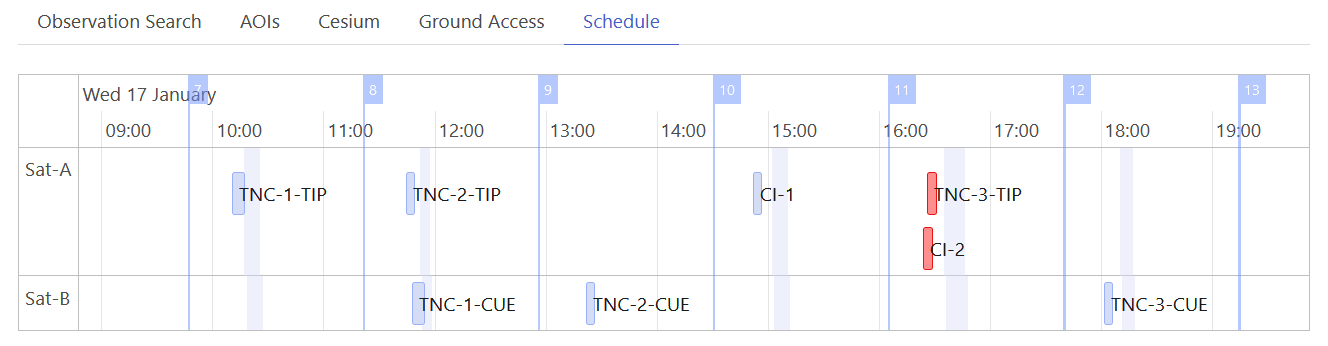
\includegraphics[width=\textwidth]{obs-conf-schedule.png} 
    \caption{Example Schedule for Plan-2}
    \label{fig:obs-conf-schedule}
\end{figure}

An example schedule can be seen in Figure~\ref{fig:obs-conf-schedule} for
Plan-2. Plan-2 was selected because there are more opportunities and there is
some time between an \gls{aoi} access and a ground access. Here, there are five
observations scheduled, 3 Tip-and-Cue Imaging observations and 2 Course Imaging
observations. The first Tip-and-Cue observation, \texttt{TNC-1-TIP}, begins at
10:10AM on Jan 17, in pass 7. Here, Sat-A begins its first tip pass over the
\gls{aoi}.  This is immediately followed by a ground contact for both
satellites with the Weilheim station. This is represented by the light grey
vertical bar.  Currently, ground contact events have not been included in the
schedule as part of an observation but this will be done in the future.  The
cue observation, \texttt{TNC-1-CUE}, happens on the next pass at 11:43AM on Jan
17.  That concludes the first observation.

While Sat-B performs the cue pass of the first observation, Sat-A begins
another observation simultaneously. Sat-B does not rely on Sat-A during a pass
so Sat-A can begin an observation as it pleases. With respect to how
observations are defined, this is acceptable, but it may conflict with the
mission's data budget. So, while the schedule does not report that there is a
conflict, in the future, another rule may be added that deals with this case.

Next, are the two Coarse Imaging Observations, \texttt{CI-1} and \texttt{CI-2},
which can be seen at 2:51PM and 4:22PM\@. The first is a legal observation but
the second conflicts with the last Tip-and-Cue observation at 4:25PM\@. The
scheduler recognizes this time conflict and highlights both events in red,
signifying to the operator that these two events must be changed before
continuing.

\subsection{Time-Tag Command Generation}\label{sec:ttc-gen}

The last stage of the \gls{pops} workflow is \gls{ttc} generation.  At this
point, the operator has created a plan that suits their own needs as well as
their customer’s needs, the plan has been validated, and all that remains is
generating \glspl{ttc} to be uploaded to their specific spacecraft.  Depending
on the observation mode, not all events have commands to be generated. In
Plan-2's schedule, commands may be only generated for the Sat-A events because
we may command it to do coarse imaging in all cases. The Sat-B events cannot
generate \glspl{ttc}. This is because for the Tip-and-Cue observation mode, on
the first pass, we may command the satellite to begin capturing wide-view
images.  But, on the next pass, we cannot command the satellite to image
potential targets as we cannot know where they will be a priori. It is known
that new commands will be generated between the first and second pass and, from
a planning perspective, this is handled with the scheduler. The time when these
inter-pass commands will be executed will lie within the second-pass event. In
this way, no other \glspl{ttc} should conflict with the automatically generated
commands because if they were scheduled for that time, they would conflict. 

To generate \glspl{ttc}, templates are combined and populated based on the
observation and the configuration parameters specified when creating the
observation. For example, one parameter may be the duration for which Sat-A
captures images. This value would then be set to an offset parameter in the
templates. 

\begin{figure}[h] 
    \centering
    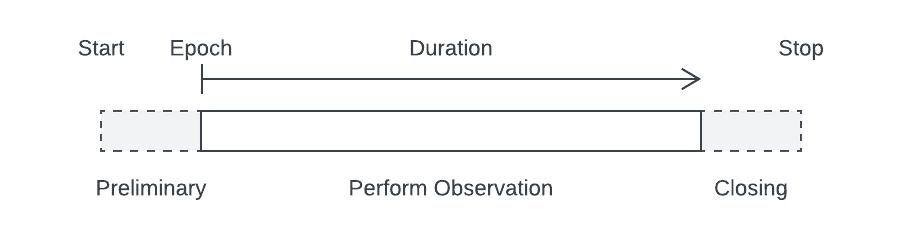
\includegraphics[width=0.7\textwidth]{timing_diagram.png} 
    \label{fig:timing} 
    \caption{Timing Diagram}
\end{figure}

The generation process is straightforward and specific to each observation mode
on each satellite. But, there are some intricacies worth noting. Firstly, when
creating an observation, the operator only specifies a duration because that is
all they are concerned with.  Generally, for any observation, there are some
preliminary and closing commands. These commands cannot happen instantaneously
and may require some non-negligible margin. It is for this reason that each
event is subdivided into separate timing components.  This can be seen in
Figure~\ref{fig:timing}. The start and stop times are the same as the event’s
start and stop but they specify when the first \gls{ttc} is executed and when
the final \gls{ttc} has concluded its execution respectively.  The epoch is the
time when the satellite begins sensing for an observation mode and the duration
is the period after which the sensing is performed. As part of the \gls{ttc}
generation capabilities, these timings can be determined programmatically by
evaluating the templates for each observation. As such, when an observation is
created by the operator in the observation configuration stage, they specify
the epoch and the duration, and the \gls{ttc} generator determines the start
and stop times. The process of generating \glspl{ttc} is still under
development and requires an intimate knowledge of the mission it is being
developed for. 




